\documentclass[border=10pt]{standalone}
\usepackage{tikz}
\usetikzlibrary{shapes.geometric}
\usetikzlibrary{arrows.meta,arrows}
\begin{document}

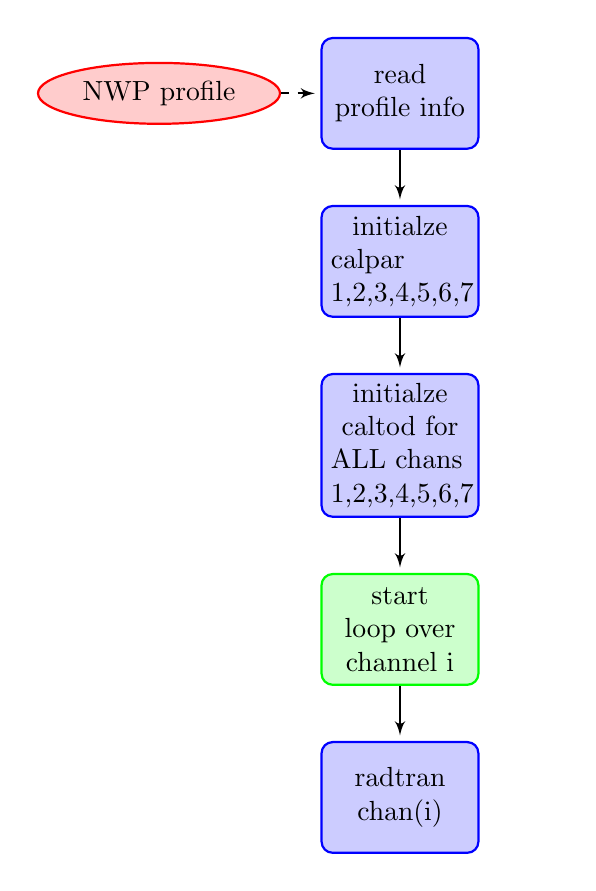
\begin{tikzpicture}
[auto,
decision/.style={diamond, draw=blue, thick, fill=blue!20,
text width=4.5em,align=flush center,
inner sep=1pt},
block/.style ={rectangle, draw=blue, thick, fill=blue!20,
text width=5em,align=center, rounded corners,
minimum height=4em},
blockG/.style ={rectangle, draw=green, thick, fill=green!20,
text width=5em,align=center, rounded corners,
minimum height=4em},
line/.style ={draw, thick, -latex',shorten >=2pt},
cloud/.style ={draw=red, thick, ellipse,fill=red!20,
minimum height=2em}]
\matrix [column sep=5mm,row sep=7mm]
{
% row 1  has three thingies
\node [cloud]  (nwp)  {NWP profile}; &
\node [block] (init) {read profile info}; & \\
% row 2 has a blank thingy and another thingy and a blank thigy
& \node [block] (calpar)    {initialze calpar \newline 1,2,3,4,5,6,7}; & \\
% row 3
& \node [block] (caltod)  {initialze caltod for ALL chans \newline 1,2,3,4,5,6,7}; & \\
% row 4
& \node [blockG] (loop)       {start loop over channel i}; & & \\
% row 5
& \node [block] (radtrans) {radtran chan(i)}; & \\
};
\begin{scope}[every path/.style=line]
\path [dashed] (nwp) -- (init);
\path (init) -- (calpar);
\path (calpar) -- (caltod);
\path (caltod) -- (loop);
\path (loop) -- (radtrans);
\end{scope}
\end{tikzpicture}

\end{document} 
